\begin{name}
	{\tenchude}{\tendethi}{LỚP TOÁN THẦY PHÁT}{\thoigian}
\end{name}
\setcounter{ex}{0}\setcounter{bt}{0}
\Opensolutionfile{ans}[ans/ans-2-TT-9-LienTruongNgheAn-23]
\begin{ex}%[Thi thử tốt nghiệp - Liên trường Nghệ An-23]%[Nguyễn Đăng Tuấn - 12-EX6-2023]%[2D3Y1-1]
	Cho hàm số $f(x)=2^x+\sin x$. Khẳng định nào sau đây đúng?
	\choice
	{$\displaystyle\int{f(x)\mathrm{\,d}x}=\dfrac{2^x}{\ln 2}+\cos x+C$}
	{$\displaystyle\int{f(x)\mathrm{\,d}x}=2^x\cdot\ln 2+\cos x+C$}
	{$\displaystyle\int{f(x)\mathrm{\,d}x}=2^x\cdot \ln 2-\cos x+C$}
	{\True $\displaystyle\int{f(x)\mathrm{\,d}x}=\dfrac{2^x}{\ln 2}-\cos x+C$}
	\loigiai{
		Ta có $\displaystyle\int{f(x)\mathrm{\,d}x}=\displaystyle\int{(2^x+\sin x)}\mathrm{\,d}x=\dfrac{2^x}{\ln 2}-\cos x+C$.
	}
\end{ex}

\begin{ex}%[Thi thử tốt nghiệp - Liên trường Nghệ An-23]%[Nguyễn Đăng Tuấn - 12-EX6-2023]%[2D1Y4-3]
	\immini{Cho hàm số $y=\dfrac{ax+b}{cx+d}$ có đồ thị là đường cong như hình bên. Toạ độ giao điểm của hai đường tiệm cận đứng và tiệm cận ngang của đồ thị là
	\choice
	{$(2;1)$}
	{$(1;-1)$}
	{\True $(-1;1)$}
	{$(2;-2)$}
}{\begin{tikzpicture}[scale=.5,>=stealth, font=\footnotesize, line join=round, line cap=round]
\def\a{1} \def\b{-2} \def\c{1} \def\d{1} % Hệ số
\def\xmin{-5} \def\xmax{4}
\def\ymin{-4} \def\ymax{4}
\draw[->] (\xmin,0)--(\xmax,0) node [below]{$x$};
\draw[->] (0,\ymin)--(0,\ymax) node [left]{$y$};
\node at (0,0) [below right]{$O$};
\clip (\xmin+0.1,\ymin+0.1) rectangle (\xmax-0.1,\ymax-0.1);
\draw[smooth,samples=300,domain=\xmin:(-\d/\c-0.1)] plot(\x,{(\a*(\x)+\b)/(\c*(\x)+\d)});
\draw[smooth,samples=300,domain=(-\d/\c+0.1:\xmax)] plot(\x,{(\a*(\x)+\b)/(\c*(\x)+\d)});
\draw[dashed] (-\d/\c,\ymin)--(-\d/\c,\ymax);
\draw[dashed] (\xmin,\a/\c)--(\xmax,\a/\c);
\draw[fill=black] (-1,0) node[shift={(-125:.4)}]{$-1$} circle(1pt);
\draw[fill=black] (0,1) node[shift={(45:.2)}]{$1$} circle(1pt);
\draw[fill=black] (0,-2) node[shift={(0:.3)}]{$-2$} circle(1pt);
\draw[fill=black] (2,0) node[shift={(90:.2)}]{$2$} circle(1pt);
\end{tikzpicture}}
	\loigiai{
		Dựa vào đồ thị hàm số ta thấy đường tiệm cận đứng $x=-1$, đường tiệm cận ngang $y=1$.\\
		Suy ra giao điểm của hai đường tiệm cận là $(-1;1)$.
	}
\end{ex}

\begin{ex}%[Thi thử tốt nghiệp - Liên trường Nghệ An-23]%[Nguyễn Đăng Tuấn - 12-EX6-2023]%[2D4Y1-1]
	Gọi $x$ là phần thực của số phức $z=4-2i$. Khi đó, $2x$ bằng
	\choice
	{$4$}
	{$4i$}
	{$-4$}
	{\True $8$}
	\loigiai{
		Số phức $z=4-2i$ có phần thực $x=4$, suy ra $2x=2\cdot4=8$.
	}
\end{ex}

\begin{ex}%[Thi thử tốt nghiệp - Liên trường Nghệ An-23]%[Nguyễn Đăng Tuấn - 12-EX6-2023]%[2D1Y5-1]
	\immini{Hàm số nào trong các hàm số sau có đồ thị như hình vẽ bên dưới?
	\choice
	{\True $y=\dfrac{x-1}{x+1}$}
	{$y=\dfrac{1-x}{x+1}$}
	{$y=x^4-2x^2+1$}
	{$y=x^3-3x+1$}
}{\begin{tikzpicture}[scale=.5,>=stealth, font=\footnotesize, line join=round, line cap=round]
\def\a{1} \def\b{-1} \def\c{1} \def\d{1} % Hệ số
\def\xmin{-5} \def\xmax{4}
\def\ymin{-4} \def\ymax{4}
\draw[->] (\xmin,0)--(\xmax,0) node [below]{$x$};
\draw[->] (0,\ymin)--(0,\ymax) node [left]{$y$};
\node at (0,0) [below left]{$O$};
\clip (\xmin+0.1,\ymin+0.1) rectangle (\xmax-0.1,\ymax-0.1);
\draw[smooth,samples=300,domain=\xmin:(-\d/\c-0.1)] plot(\x,{(\a*(\x)+\b)/(\c*(\x)+\d)});
\draw[smooth,samples=300,domain=(-\d/\c+0.1:\xmax)] plot(\x,{(\a*(\x)+\b)/(\c*(\x)+\d)});
\draw[dashed] (-\d/\c,\ymin)--(-\d/\c,\ymax);
\draw[dashed] (\xmin,\a/\c)--(\xmax,\a/\c);
\draw[fill=black] (-1,0) node[shift={(-125:.4)}]{$-1$} circle(1pt);
\draw[fill=black] (0,1) node[shift={(45:.2)}]{$1$} circle(1pt);
\draw[fill=black] (0,-1) node[shift={(0:.3)}]{$-1$} circle(1pt);
\draw[fill=black] (1,0) node[shift={(90:.2)}]{$1$} circle(1pt);
\end{tikzpicture}}
	\loigiai{
		Dựa vào đồ thị hàm số ta thấy đường tiệm cận đứng $x=-1$, đường tiệm cận ngang $y=1$.\\
		Vậy đồ thị hàm số đó là $y=\dfrac{x-1}{x+1}$.
	}
\end{ex}

\begin{ex}%[Thi thử tốt nghiệp - Liên trường Nghệ An-23]%[Nguyễn Đăng Tuấn - 12-EX6-2023]%[2D3Y2-1]
	Cho $\displaystyle\int{\dfrac{1}{x^2}\mathrm{\,d}x=f(x)+C}$. Khẳng định nào sau đây đúng?
	\choice
	{\True $f(x)=-\dfrac{1}{x}$}
	{$f(x)=\dfrac{1}{x}$}
	{$f(x)=\ln x$}
	{$f(x)=\ln x^2$}
	\loigiai{
		Ta có $\displaystyle\int{\dfrac{1}{x^2}\mathrm{\,d}x=-\dfrac{1}{x}+C}$ mà $\displaystyle\int{\dfrac{1}{x^2}\mathrm{\,d}x=f(x)+C}$, suy ra $f(x)=-\dfrac{1}{x}$.\\
		Vậy $f(x)=-\dfrac{1}{x}$.
	}
\end{ex}

\begin{ex}%[Thi thử tốt nghiệp - Liên trường Nghệ An-23]%[Nguyễn Đăng Tuấn - 12-EX6-2023]%[2D2Y4-1]
	Tập xác định của hàm số $y=\log_2(x-1)$ là
	\choice
	{$(-\infty;1)$}
	{$(0;+\infty)$}
	{$[1;+\infty)$}
	{\True $(1;+\infty)$}
	\loigiai{
		Điều kiện $x-1>0\Leftrightarrow x>1$.\\
		Vậy tập xác định của hàm số là $\mathscr{D} = (1;+\infty)$.
	}
\end{ex}

\begin{ex}%[Thi thử tốt nghiệp - Liên trường Nghệ An-23]%[Nguyễn Đăng Tuấn - 12-EX6-2023]%[2H3Y3-1]
	Trong không gian $Oxyz$, cho đường thẳng $d$ có phương trình $\dfrac{x-2}{3}=\dfrac{y+1}{-2}=\dfrac{z}{4}$. Tọa độ một véc-tơ chỉ phương của đường thẳng $d$ là
	\choice
	{$(2;-1;0)$}
	{$(-2;1;0)$}
	{\True $(3;-2;4)$}
	{$(-3;-2;4)$}
	\loigiai{
		Một véc-tơ chỉ phương của đường thẳng $d$ là $(3;-2;4)$.
	}
\end{ex}

\begin{ex}%[Thi thử tốt nghiệp - Liên trường Nghệ An-23]%[Nguyễn Đăng Tuấn - 12-EX6-2023]%[2D3B2-1]
	Nếu $\displaystyle\int\limits_1^3{f(x)\mathrm{\,d}x=8}$ và $\displaystyle\int\limits_1^5{f(x)\mathrm{\,d}x=-4}$ thì $\displaystyle\int\limits_3^5{f(x)\mathrm{\,d}x}$ bằng
	\choice
	{\True $-12$}
	{$12$}
	{$4$}
	{$-4$}
	\loigiai{
		Ta có $\displaystyle\int\limits_3^5{f(x)\mathrm{\,d}x}=\displaystyle\int\limits_1^5{f(x)\mathrm{\,d}x}-\displaystyle\int\limits_1^3{f(x)\mathrm{\,d}x}=-4-8=-12$.
	}
\end{ex}

\begin{ex}%[Thi thử tốt nghiệp - Liên trường Nghệ An-23]%[Nguyễn Đăng Tuấn - 12-EX6-2023]%[2D4Y1-1]
	Cho số phức $z=3-4i$, mô-đun số phức $z$ bằng
	\choice
	{\True $5$}
	{$\sqrt{12}$}
	{$\sqrt{7}$}
	{$1$}
	\loigiai{
	Ta có $|z|=\sqrt{3^2+4^2}=5$.
	}
\end{ex}

\begin{ex}%[Thi thử tốt nghiệp - Liên trường Nghệ An-23]%[Nguyễn Đăng Tuấn - 12-EX6-2023]%[2D3Y2-1]
	Nếu $\displaystyle\int\limits_2^4{f(x)\mathrm{\,d}x=5}$ thì ${\displaystyle\int\limits_2^4{\left[1+f(x)\right]\mathrm{\,d}x}}$ bằng
	\choice
	{$11$}
	{$6$}
	{\True $7$}
	{$8$}
	\loigiai{
	Ta có $\displaystyle\int\limits_2^4{\left[1+f(x)\right]\mathrm{\,d}x}=\displaystyle\int\limits_2^4{1\mathrm{\,d}x}+\displaystyle\int\limits_2^4{f(x)\mathrm{\,d}x}=2+5=7$.
	}
\end{ex}

\begin{ex}%[Thi thử tốt nghiệp - Liên trường Nghệ An-23]%[Nguyễn Đăng Tuấn - 12-EX6-2023]%[2H2Y1-2]
	Cho hình trụ có đường kính đáy bằng $2a$, chiều cao bằng $a$. Diện tích toàn phần của hình trụ bằng
	\choice
	{$5\pi a^2$}
	{\True $4\pi a^2$}
	{$3\pi a^2$}
	{$6\pi a^2$}
	\loigiai{
		Hình trụ có đường kính đáy bằng $2a\Rightarrow r=a$.\\
		Diện tích toàn phần của hình trụ là $S=2\pi rh+2\pi r^2=2\pi\cdot a\cdot a+2\pi\cdot a^2=4\pi a^2$.
	}
\end{ex}

\begin{ex}%[Thi thử tốt nghiệp - Liên trường Nghệ An-23]%[Nguyễn Đăng Tuấn - 12-EX6-2023]%[2H1Y3-2]
	Một khối lập phương có diện tích bốn mặt bằng $36$, thể tích của khối lập phương bằng
	\choice
	{$18$}
	{\True $27$}
	{$54$}
	{$12$}
	\loigiai{
		Gọi cạnh của hình lập phương bằng $x$.\\
		Ta có diện tích bốn mặt của hình lập phương bằng $4x^2=36\Leftrightarrow x=3$.\\
		Thể tích của khối lập phương bằng $x^3=3^3=27$.
	}
\end{ex}

\begin{ex}%[Thi thử tốt nghiệp - Liên trường Nghệ An-23]%[Nguyễn Đăng Tuấn - 12-EX6-2023]%[2H3Y2-4]
	Trong không gian $Oxyz$, cho mặt phẳng $(P)$ có phương trình $3x-y+z-5=0$. Điểm nào sau đây thuộc mặt phẳng $(P)$?
	\choice
	{$Q(1;-2;4)$}
	{\True $N(1;-2;0)$}
	{$M(0;0;-5)$}
	{$P(0;5;0)$}
	\loigiai{
		Thay tọa độ các điểm vào mặt phẳng $(P)$ ta có $N(1;-2;0)\in (P)$.
	}
\end{ex}

\begin{ex}%[Thi thử tốt nghiệp - Liên trường Nghệ An-23]%[Nguyễn Đăng Tuấn - 12-EX6-2023]%[1D3Y4-3]
	Cho cấp số nhân $(u_n)$ với $u_1=-2$ và công bội $q=\dfrac{3}{2}$. Giá trị của $u_3$ bằng
	\choice
	{\True $-\dfrac{9}{2}$}
	{$-\dfrac{9}{8}$}
	{$\dfrac{9}{8}$}
	{$\dfrac{9}{2}$}
	\loigiai{
		Ta có $u_3=u_1\cdot q^2=-2\cdot \left(\dfrac{3}{2}\right)^2=-\dfrac{9}{2}$.
	}
\end{ex}

\begin{ex}%[Thi thử tốt nghiệp - Liên trường Nghệ An-23]%[Nguyễn Đăng Tuấn - 12-EX6-2023]%[2D2Y2-2]
	Trên $(0;+\infty )$, đạo hàm của hàm số $y=x^{\tfrac{4}{3}}$ là
	\choice
	{$y'=\dfrac{3}{7}x^{\tfrac{7}{3}}$}
	{\True $y'=\dfrac{4}{3}x^{\tfrac{1}{3}}$}
	{$y'=\dfrac{7}{3}x^{\tfrac{7}{3}}$}
	{$y'=\dfrac{3}{4}x^{\tfrac{1}{3}}$}
	\loigiai{
		Ta có $y=x^{\tfrac{4}{3}}\Rightarrow y'=\dfrac{4}{3}x^{\tfrac{1}{3}}$.
	}
\end{ex}

\begin{ex}%[Thi thử tốt nghiệp - Liên trường Nghệ An-23]%[Nguyễn Đăng Tuấn - 12-EX6-2023]%[1D2Y2-1]
	Kí hiệu $\mathrm{C}_5^2$ là
	\choice
	{Số các tổ hợp chập $5$ của $2$}
	{\True Số các tổ hợp chập $2$ của $5$}
	{Tổ hợp chập $2$ của $5$}
	{Tổ hợp chập $5$ của $2$}
	\loigiai{
		Kí hiệu $\mathrm{C}_5^2$ là số các tổ hợp chập $2$ của $5$.
	}
\end{ex}

\begin{ex}%[Thi thử tốt nghiệp - Liên trường Nghệ An-23]%[Nguyễn Đăng Tuấn - 12-EX6-2023]%[2D2Y6-1]
	Tập nghiệm của bất phương trình $4^x<16$ là
	\choice
	{$(-\infty; 0)$}
	{$(-\infty;2]$}
	{$(0; 2)$}
	{\True $(-\infty; 2)$}
	\loigiai{
	Ta có $4^x<16\Leftrightarrow 4^x<4^2\Leftrightarrow x<2$.\\
	Vậy tập nghiệm của bất phương trình là $(-\infty; 2)$.
	}
\end{ex}

\begin{ex}%[Thi thử tốt nghiệp - Liên trường Nghệ An-23]%[Nguyễn Đăng Tuấn - 12-EX6-2023]%[2D1Y2-2]
	\immini{Cho hàm số $y=ax^3+bx^2+cx+d$, $(a \neq 0)$ có đồ thị là đường cong trong hình bên. Điểm cực tiểu của đồ thị hàm số đã cho có tọa độ là
	\choice
	{$(-2; 1)$}
	{$(2;-1)$}
	{\True $(1;-2)$}
	{$(-1; 2)$}
}{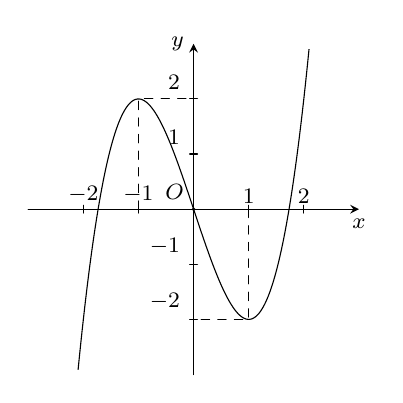
\begin{tikzpicture}[scale=.7, font=\footnotesize, line join=round, line cap=round,>=stealth]
\def\xmin{-3} \def\xmax{3}
\def\ymin{-3} \def\ymax{3} 
\draw[->] (\xmin,0)--(\xmax,0) node [below]{$x$};
\draw[->] (0,\ymin)--(0,\ymax) node [left]{$y$};
\node at (0,0) [above left]{$O$};
\foreach \x in {-2,-1,1,2}
\draw[shift={(\x,0)},color=black] (0pt,2pt) -- (0pt,-2pt) node[above]{$\x$};
\foreach \y in {-2,-1,1,2}
\draw[shift={(0,\y)},color=black] (2pt,0pt) -- (-2pt,0pt) node[above left]{$\y$};
\clip (\xmin+0.1,\ymin+0.1) rectangle (\xmax-0.1,\ymax-0.1);
\draw[smooth,samples=300] plot(\x,{(\x)^3-3*(\x)});
\fill (0,0) circle (1.0pt);
\draw[dashed] (-1,0)|-(0,2) (1,0)|-(0,-2);
\end{tikzpicture}}
	\loigiai{
		Điểm cực tiểu của đồ thị hàm số đã cho là $(1;-2)$.
	}
\end{ex}

\begin{ex}%[Thi thử tốt nghiệp - Liên trường Nghệ An-23]%[Nguyễn Đăng Tuấn - 12-EX6-2023]%[2H1Y3-2]
	Cho tứ diện $ABCD$ biết rằng khoảng cách từ điểm $A$ đến $(BCD)$ bằng $2$ và diện tích tam giác $BCD$ bằng $6$. Thể tích khối tứ diện đã cho bằng
	\choice
	{\True $4$}
	{$6$}
	{$12$}
	{$3$}
	\loigiai{
		Thể tích khối tứ diện đã cho bằng $V=\dfrac{1}{3}\cdot S_{BCD}\cdot \mathrm{d}(A,(BCD))=\dfrac{1}{3}\cdot 6\cdot 2=4$.
	}
\end{ex}

\begin{ex}%[Thi thử tốt nghiệp - Liên trường Nghệ An-23]%[Nguyễn Đăng Tuấn - 12-EX6-2023]%[2H3B2-5]
	Trong không gian $Oxyz$, góc giữa hai mặt phẳng $(\alpha)\colon x+z-1=0$ và $(\beta)\colon y+3=0$ bằng
	\choice
	{\True $90^\circ$}
	{$60^\circ$}
	{$45^\circ$}
	{$0^\circ$}
	\loigiai{
		Mặt phẳng $(\alpha)\colon x+z-1=0$ và $(\beta)\colon y+3=0$ có véc-tơ pháp tuyến lần lượt là $\overrightarrow{n}_1=(1;0;1)$ và $\overrightarrow{n}_2=(0;1;0)$.\\
		Ta có $\overrightarrow{n}_1\cdot\overrightarrow{n}_2=0\Leftrightarrow \overrightarrow{n}_1\perp \overrightarrow{n}_2$. Suy ra $(\alpha )\perp (\beta )$.\\
		Vậy góc giữa hai mặt phẳng $(\alpha )$ và $(\beta )$ bằng $90^\circ$.
	}
\end{ex}

\begin{ex}%[Thi thử tốt nghiệp - Liên trường Nghệ An-23]%[Nguyễn Đăng Tuấn - 12-EX6-2023]%[2D2B6-1]
	Tập nghiệm của bất phương trình $\ln \dfrac{1}{2x-1}\ge 0$ là
	\choice
	{$\left(\dfrac{1}{2};+\infty\right)$}
	{$\left(\dfrac{1}{2};1\right)$}
	{\True $\left(\dfrac{1}{2};1\right]$}
	{$(-\infty;1)$}
	\loigiai{
		Điều kiện $\dfrac{1}{2x-1}>0\Leftrightarrow 2x-1>0\Leftrightarrow x>\dfrac{1}{2}$.\\
		Ta có $\ln \dfrac{1}{2x-1}\ge 0\Leftrightarrow \dfrac{1}{2x-1}\ge 1\Leftrightarrow 2x-1\le 1\Leftrightarrow x\le 1$.\\
		Kết hợp với điều kiện ta có $\dfrac{1}{2}<x\le 1$.\\
		Vậy tập nghiệm của bất phương trình là $\left(\dfrac{1}{2};1\right]$.
	}
\end{ex}

\begin{ex}%[Thi thử tốt nghiệp - Liên trường Nghệ An-23]%[Nguyễn Đăng Tuấn - 12-EX6-2023]%[2D4B2-2]
	Cho hai số phức $z_1=6+3i$ và $z_2=1-5i$. Trong mặt phẳng $(Oxy)$, tìm tọa độ điểm biểu diễn số phức $z=z_1+z_2$.
	\choice
	{$M(7;2)$}
	{$N(1;4)$}
	{$Q(7;-8)$}
	{\True $P(7;-2)$}
	\loigiai{
		Ta có $z=z_1+z_2=(6+3i)+(1-5i)=7-2i$.\\
		Vậy tọa độ điểm biểu diễn số phức $z=z_1+z_2$ là điểm $P(7;-2)$.
	}
\end{ex}

\begin{ex}%[Thi thử tốt nghiệp - Liên trường Nghệ An-23]%[Nguyễn Đăng Tuấn - 12-EX6-2023]%[2H3B1-3]
	Trong không gian $Oxyz$, cho mặt cầu $(S)$ có phương trình $x^2+y^2+z^2-2x-4y-2z+2=0$. Bán kính của mặt cầu bằng
	\choice
	{$6$}
	{$4$}
	{\True $2$}
	{$\sqrt{6}$}
	\loigiai{
		Gọi $I$ và $R$ lần lượt là tâm và bán kính của mặt cầu $(S)$.\\
		Ta có $I(1;2;1)$. Vậy $R=\sqrt{1^2+2^2+1^2-2}=2$.
	}
\end{ex}

\begin{ex}%[Thi thử tốt nghiệp - Liên trường Nghệ An-23]%[Nguyễn Đăng Tuấn - 12-EX6-2023]%[2D1Y4-1]
	Tiệm cận ngang của đồ thị hàm số $y=\dfrac{x+1}{5x-2}$ là đường thẳng có phương trình là
	\choice
	{$y=\dfrac{2}{5}$}
	{$y=-\dfrac{1}{5}$}
	{$y=-\dfrac{2}{5}$}
	{\True $y=\dfrac{1}{5}$}
	\loigiai{
		Tập xác định $\mathscr{D} = \mathbb{R}\setminus \left\{\dfrac{2}{5}\right\}$.\\
		Ta có
		$\lim\limits_{x\to+\infty}y=\lim\limits_{x\to+\infty}\dfrac{x+1}{5x-2}=\dfrac{1}{5}$ và $\lim\limits_{x\to-\infty}y=\lim\limits_{x\to-\infty}\dfrac{x+1}{5x-2}=\dfrac{1}{5}$.\\
		Vậy $y=\dfrac{1}{5}$ là tiệm cận ngang của đồ thị hàm số.
	}
\end{ex}

\begin{ex}%[Thi thử tốt nghiệp - Liên trường Nghệ An-23]%[Nguyễn Đăng Tuấn - 12-EX6-2023]%[2H3B2-7]
	Cho $(P)$ là một mặt phẳng đi qua tâm của mặt cầu $S(O;R)$ và cắt mặt cầu theo một đường tròn có bán kính $R'$. Khẳng định nào sau đây đúng?
	\choice
	{$R'>R$}
	{$0<R'<R$}
	{$R>R'$}
	{\True $R=R'$}
	\loigiai{
		Ta có mặt phẳng $(P)$ đi qua tâm $O$, suy ra mặt phẳng $(P)$ cắt mặt cầu $S(O;R)$ theo giao tuyến là đường tròn lớn.\\
		Vậy $R=R'$.
	}
\end{ex}

\begin{ex}%[Thi thử tốt nghiệp - Liên trường Nghệ An-23]%[Nguyễn Đăng Tuấn - 12-EX6-2023]%[1D2B5-2]
	Một hộp chứa $21$ quả cầu gồm $9$ quả cầu xanh được đánh số từ $1$ đến $9$, $7$ quả cầu đỏ được đánh số từ $1$ đến $7$ và $5$ quả cầu màu vàng được đánh số từ $1$ đến $5$. Chọn ngẫu nhiên ba quả từ hộp đó, xác xuất để ba quả được chọn có đủ ba màu và đôi một khác số nhau là
	\choice
	{$\dfrac{9}{38}$}
	{$\dfrac{9}{19}$}
	{\True $\dfrac{3}{19}$}
	{$\dfrac{24}{133}$}
	\loigiai{
		Ta có $n(\Omega )=\mathrm{C}_{21}^3=1330$.\\
		Gọi $A$ là biến cố chọn ba quả cầu đủ ba màu và đôi một khác số nhau.
		\begin{itemize}
			\item Chọn $1$ quả cầu màu vàng $\mathrm{C}_5^1$.
			\item Chọn $1$ quả cầu màu đỏ $\mathrm{C}_6^1$.
			\item Chọn $1$ quả cầu màu xanh $\mathrm{C}_7^1$.
		\end{itemize}
		$\Rightarrow n(A)=\mathrm{C}_5^1\cdot \mathrm{C}_6^1\cdot \mathrm{C}_7^1=210$.\\
		$\Rightarrow \mathrm{P}(A)=\dfrac{n(A)}{n(\Omega )}=\dfrac{210}{1330}=\dfrac{3}{19}$.
	}
\end{ex}

\begin{ex}%[Thi thử tốt nghiệp - Liên trường Nghệ An-23]%[Nguyễn Đăng Tuấn - 12-EX6-2023]%[2D3B3-3]
	Tính thể tích khối tròn xoay thu được khi quay hình phẳng giới hạn bởi hai đường $y=x^2+2$ và $y=3$ quay quanh trục $Ox$.
	\choice
	{$\dfrac{16\pi}{15}$}
	{\True $\dfrac{104\pi}{15}$}
	{$\dfrac{56\pi}{15}$}
	{$\dfrac{16}{15}$}
	\loigiai{
		Ta có phương trình hoành độ giao điểm $x^2+2=3\Rightarrow x=\pm 1$.\\
		Khi đó $V=\pi \displaystyle\int\limits_{-1}^1{\left|(x^2+2)^2-3^2\right|\mathrm{\,d}x}=\dfrac{104\pi}{15}$.
	}
\end{ex}

\begin{ex}%[Thi thử tốt nghiệp - Liên trường Nghệ An-23]%[Nguyễn Đăng Tuấn - 12-EX6-2023]%[2D1Y2-2]
	\immini{Cho hàm số bậc bốn $y=f(x)$ có đồ thị là đường cong hình bên. Giá trị cực tiểu của hàm số đã cho là
	\choice
	{$2$}
	{\True $1$}
	{$0$}
	{$-1$}
}{\begin{tikzpicture}[scale=1, font=\footnotesize, line join=round, line cap=round,>=stealth]
\def\xmin{-3} \def\xmax{3}
\def\ymin{-1} \def\ymax{3} 
\draw[->] (\xmin,0)--(\xmax,0) node [below]{$x$};
\draw[->] (0,\ymin)--(0,\ymax) node [left]{$y$};
\node at (0,0) [above left]{$O$};
\foreach \x in {-2,-1,1,2}
\draw[shift={(\x,0)},color=black] (0pt,2pt) -- (0pt,-2pt) node[below]{$\x$};
\foreach \y in {1,2}
\draw[shift={(0,\y)},color=black] (2pt,0pt) -- (-2pt,0pt) node[below left]{$\y$};
\clip (\xmin+0.1,\ymin+0.1) rectangle (\xmax-0.1,\ymax-0.1);
\draw[smooth,samples=300] plot(\x,{-(\x)^4+2*(\x)^2+1});
\fill (0,0) circle (1.0pt);
\draw[dashed] (-1,0)|-(0,2) (1,0)|-(0,2);
\end{tikzpicture}}
	\loigiai{
		Quan sát đồ thị hàm số $y=f(x)$ ta thấy giá trị cực tiểu của hàm số là $y=1$.
	}
\end{ex}

\begin{ex}%[Thi thử tốt nghiệp - Liên trường Nghệ An-23]%[Nguyễn Đăng Tuấn - 12-EX6-2023]%[2D2B5-3]
	Tổng các nghiệm của phương trình $\log^2x-\log x-2=0$ bằng
	\choice
	{$\dfrac{1001}{100}$}
	{$101$}
	{\True $\dfrac{1001}{10}$}
	{$1$}
	\loigiai{
		Ta có $\log^2x-\log x-2=0\Leftrightarrow \hoac{
			& \log x=2 \\ 
			& \log x=-1 \\}\Leftrightarrow \hoac{
			& x_1=100 \\ 
			& x_2=\dfrac{1}{10} \\}$ $\Rightarrow x_1+x_2=\dfrac{1001}{10}$.
	}
\end{ex}

\begin{ex}%[Thi thử tốt nghiệp - Liên trường Nghệ An-23]%[Nguyễn Đăng Tuấn - 12-EX6-2023]%[2D1B1-1]
	Cho hàm số $y=f(x)$ có đạo hàm $f'(x)=x^2(2-x)$ với mọi $x\in \mathbb{R}$. Hàm số đã cho nghịch biến trên khoảng nào dưới đây?
	\choice
	{$(0;2)$}
	{$(-\infty;0)$}
	{\True $(2;+\infty)$}
	{$(-\infty;2)$}
	\loigiai{
	Tập xác định $\mathscr{D} = \mathbb{R}$.\\ 
	Ta có $f'(x)=0 \Leftrightarrow \hoac{&x=0\\&x=2.}$\\
	Bảng xét dấu
	\begin{center}
		
\begin{tikzpicture}
		\tkzTabInit[nocadre=false,lgt=1.5,espcl=3,deltacl=.6]
		{$x$/0.6,$f'(x)$/0.6}
		{$-\infty$,$0$,$2$,$+\infty$}
		\tkzTabLine{,+,$0$,+,$0$,-,}
		\end{tikzpicture}
	\end{center}
	Dựa vào bảng xét dấu, hàm số nghịch biến trong khoảng $(2;+\infty)$.
	}
\end{ex}

\begin{ex}%[Thi thử tốt nghiệp - Liên trường Nghệ An-23]%[Nguyễn Đăng Tuấn - 12-EX6-2023]%[2D1B1-2]
	Cho hàm số $f(x)$ có bảng biến thiên như sau
	\begin{center}
		
\begin{tikzpicture}
		\tkzTabInit[nocadre=false,lgt=1.5,espcl=3,deltacl=.6]
		{$x$/0.6,$f'(x)$/0.6,$f(x)$/2}
		{$-\infty$,$0$,$2$,$+\infty$}
		\tkzTabLine{,-,$0$,+,$0$,-,}
		\tkzTabVar{+/$+\infty$,-/$-1$,+/$3$,-/$-\infty$}
		\end{tikzpicture}
	\end{center}
	Hàm số đã cho đồng biến trên khoảng nào dưới đây?
	\choice
	{\True $(0;2)$}
	{$(-1;3)$}
	{$(2;+\infty )$}
	{$(-\infty;0)$}
	\loigiai{
	Dựa vào bảng biến thiên, hàm số đồng biến trên khoảng $(0;2)$.
	}
\end{ex}

\begin{ex}%[Thi thử tốt nghiệp - Liên trường Nghệ An-23]%[Nguyễn Đăng Tuấn - 12-EX6-2023]%[2D2Y3-1]
	Với $a$ là số thực dương và $a\ne 1$, $\log_aa^2$ bằng
	\choice
	{$\dfrac{1}{2}$}
	{\True $2$}
	{$\sqrt{2}$}
	{$a^2$}
	\loigiai{
		Ta có $\log_aa^2=2$.
	}
\end{ex}

\begin{ex}%[Thi thử tốt nghiệp - Liên trường Nghệ An-23]%[Nguyễn Đăng Tuấn - 12-EX6-2023]%[2D1B5-3]
	Cho hàm số $y=f(x)$ xác định trên $\mathbb{R}$ và có bảng biến thiên như sau
	\begin{center}
		
\begin{tikzpicture}
		\tkzTabInit[nocadre=false,lgt=1.5,espcl=3,deltacl=.6]
		{$x$/0.6,$f'(x)$/0.6,$f(x)$/2}
		{$-\infty$,$-1$,$3$,$+\infty$}
		\tkzTabLine{,+,$0$,-,$0$,+,}
		\tkzTabVar{-/$-\infty$,+/$4$,-/$-2$,+/$+\infty$}
		\end{tikzpicture}
	\end{center}
	Tổng các giá trị nguyên của tham số $m$ để phương trình $f(x)+3=m$ có ba nghiệm phân biệt là
	\choice
	{\True $20$}
	{$28$}
	{$27$}
	{$25$}
	\loigiai{
		Phương trình $f(x)+3=m\Leftrightarrow f(x)=m-3$.\\
		Phương trình có ba nghiệm phân biệt $\Leftrightarrow-2<m-3<4\Leftrightarrow 1<m<7$.\\
		Mà $m\in \mathbb{Z}$, suy ra $m\in \left\{2;3;4;5;6\right\}$. Tổng các giá trị $m$ là $20$.
	}
\end{ex}

\begin{ex}%[Thi thử tốt nghiệp - Liên trường Nghệ An-23]%[Nguyễn Đăng Tuấn - 12-EX6-2023]%[2H1B3-4]
	Cho khối chóp tam giác đều $S.ABC$ biết $AB=a$ và $SA=2a$. Tính chiều cao $h$ của khối chóp $S.ABC$.
	\choice
	{$h=\dfrac{a\sqrt{33}}{9}$}
	{\True $h=\dfrac{a\sqrt{33}}{3}$}
	{$h=\dfrac{a\sqrt{141}}{6}$}
	{$h=\dfrac{a\sqrt{6}}{3}$}
	\loigiai{
		\immini{Do đáy là tam giác đều nên gọi $I$ là trung điểm cạnh $BC$, khi đó $AI$ là đường cao của tam giác đáy. Chiều cao của chóp là $SO$.\\
		Theo định lý Pitago ta có $$AI=\sqrt{a^2-\dfrac{a^2}{4}}=\dfrac{a\sqrt{3}}{2},  AO=\dfrac{2}{3}AI=\dfrac{2a\sqrt{3}}{3\cdot 2}=\dfrac{a\sqrt{3}}{3}.$$
		Trong tam giác $SOA$ vuông tại $O$ ta có $$SO=\sqrt{SA^2-AO^2}=\sqrt{4a^2-\dfrac{a^2}{3}}=\dfrac{a\sqrt{33}}{3}.$$
	}{\begin{tikzpicture}[scale=1,>=stealth, font=\footnotesize, line join=round, line cap=round]
	\path%Khai báo các điểm
	(0:0) coordinate (A)
	(0:4) coordinate (C)
	(-40:2) coordinate (B)
	($(C)!.5!(B)$) coordinate (I)
	($(I)!.333!(A)$) coordinate (O)
	--++(90:3) coordinate (S)
	;
	\draw (S)--(B)--(A)--(S)--(C)--(B);
	\draw[dashed] (I)--(A)--(C) (S)--(O);
	\draw pic[draw,angle radius=2mm]{right angle=S--O--I};
	\foreach \x/\g in {A/180,B/-90,C/0,S/90,O/-90,I/-80}\fill[black] (\x) circle (1pt) +(\g:.3)node{$\x$};
	\end{tikzpicture}}
	}
\end{ex}

\begin{ex}%[Thi thử tốt nghiệp - Liên trường Nghệ An-23]%[Nguyễn Đăng Tuấn - 12-EX6-2023]%[2D4B2-4]
	Trong mặt phẳng tọa độ $Oxy$, tập hợp các điểm biểu biễn các số phức $z$ thỏa mãn $|z+3|=|\overline{z}+2i-1|$ là một đường thẳng, đường thẳng đó đi qua điểm nào dưới đây?
	\choice
	{$(1;1)$}
	{\True $(-1;1)$}
	{$(-1;-1)$}
	{$(1;-1)$}
	\loigiai{
		Đặt $z=x+yi$ $(x,y\in \mathbb{R})$ $\Rightarrow \overline{z}=x-yi$ và $M(x;y)$ là điểm biểu diễn của số phức $z$.\\
		Ta có 
		\allowdisplaybreaks
		\begin{eqnarray*}
			|z+3|=|\overline{z}+2i-1|&\Leftrightarrow& |x+yi+3|=|x-yi+2i-1|\\
			&\Leftrightarrow& |(x+3)+yi|=|(x-1)+(2-y)i|\\
			&\Leftrightarrow& \sqrt{{(x+3)}^2+y^2}=\sqrt{(x-1)^2+(2-y)^2}\\
			&\Leftrightarrow& x^2+6x+9+y^2=x^2-2x+1+y^2-4y+4\\
			&\Leftrightarrow&8x+4y+4=0\Leftrightarrow 2x+y+1=0.
		\end{eqnarray*}
		Lại có $2\cdot (-1)+1+1=0$ nên đường thẳng đi qua điểm $(-1;1)$.\\
		Vậy tập hợp các điểm biểu biễn các số phức $z$ thỏa mãn yêu cầu bài toán là đường thẳng đi qua điểm $(-1;1)$.
	}
\end{ex}

\begin{ex}%[Thi thử tốt nghiệp - Liên trường Nghệ An-23]%[Nguyễn Đăng Tuấn - 12-EX6-2023]%[2H3B3-2]
	Trong không gian với hệ toạ độ $Oxyz$, cho điểm $A(1;2;3)$ và hai mặt phẳng $(P)\colon 2x+2y+z+1=0$, $(Q)\colon 2x-y+2z-1=0$. Phương trình đường thẳng đi qua $A$, song song với $(P)$ và $(Q)$ là
	\choice
	{$\dfrac{x-1}{1}=\dfrac{y-2}{2}=\dfrac{z-3}{-6}$}
	{$\dfrac{x-1}{1}=\dfrac{y-2}{6}=\dfrac{z-3}{2}$}
	{\True $\dfrac{x-1}{5}=\dfrac{y-2}{-2}=\dfrac{z-3}{-6}$}
	{$\dfrac{x-1}{1}=\dfrac{y-2}{1}=\dfrac{z-3}{-4}$}
	\loigiai{
		Ta có $\heva{
			& \vec{n}_P=(2;2;1) \\ 
			& \vec{n}_Q=(2;-1;2)}$ và $\left[\vec{n}_P,\vec{n}_Q\right]=(5;-2;-6)$. Vì đường thẳng $d$ song song với hai mặt phẳng $(P)$ và $(Q)$, nên $d$ có véc-tơ  chỉ phương $\vec{u}=(5;-2;-6)$.\\
		Đường thẳng $d$ đi qua $A(1;2;3)$ nên có phương trình $\dfrac{x-1}{5}=\dfrac{y-2}{-2}=\dfrac{z-3}{-6}$.
	}
\end{ex}
\begin{ex}%[Thi thử tốt nghiệp - Liên trường Nghệ An-23]%[Nguyễn Đăng Tuấn - 12-EX6-2023]%[2H3B2-4]
	Trong không gian, cho điểm $A(2;-1;1)$ và điểm $A'$ là điểm đối xứng với điểm $A$ qua trục $Oz$. Điểm $A'$ nằm trên mặt phẳng nào trong các mặt phẳng dưới đây?
	\choice
	{\True $3x+2y+5z-1=0$}
	{$3x+5y+z+2=0$}
	{$2x+4y+z+1=0$}
	{$3x+4y-z-1=0$}
	\loigiai{
		Điểm $A'$ là điểm đối xứng với điểm $A$ qua trục $Oz$ suy ra $A'(-2;1;1)$.\\
		Thay tọa độ điểm $A(-2;1;1)$ vào phương trình mặt phẳng $3x+2y+5z-1=0$ ta được
		$3\cdot (-2)+2\cdot 1+5\cdot 1-1=0$ thỏa mãn.\\
		Vậy điểm $A'$ nằm trên mặt phẳng mặt phẳng có phương trình $3x+2y+5z-1=0$.
	}
\end{ex}
\begin{ex}%[Thi thử tốt nghiệp - Liên trường Nghệ An-23]%[Nguyễn Đăng Tuấn - 12-EX6-2023]%[1H3K2-3]
	Cho hình chóp tam giác $S.ABC$ có cạnh $SA$ vuông góc với mặt phẳng đáy $(ABC)$, tam giác $ABC$ vuông tại $B$, $SA=AB=a$, $BC=a\sqrt{2}$. Góc giữa hai đường thẳng $SB$ và $SC$ là
	\choice
	{$60^\circ$}
	{$30^\circ$}
	{\True $45^\circ$}
	{$90^\circ$}
	\loigiai{
		\immini{Góc $(SB,SC)=\widehat{BSC}$.\\
			Ta có $\heva{&BC\perp SA\\&BC\perp AB}\Rightarrow BC\perp SB$.\\
			$SB=\sqrt{SA^2+AB^2}=a\sqrt{2}$, suy ra tam giác $SBC$ vuông cân tại $B$ $\Rightarrow \widehat{BSC}=45^\circ $.\\
			Vậy góc giữa hai đường thẳng $SB$ và $SC$ bằng $45^\circ $.
		}{\begin{tikzpicture}[scale=1,>=stealth, font=\footnotesize, line join=round, line cap=round]
			\path%Khai báo các điểm
			(0:0) coordinate (A)
			(0:3) coordinate (C)
			(-30:1.5) coordinate (B)
			(90:2) coordinate (S)
			;
			\draw (S)--(B)--(A)--(S)--(C)--(B);
			\draw[dashed] (A)--(C);
			\draw pic[draw,angle radius=2mm]{right angle=S--A--B};
			\draw pic[draw,angle radius=2mm]{right angle=A--B--C};
			\foreach \x/\g in {A/180,B/-90,C/0,S/90}\fill[black] (\x) circle (1pt) +(\g:.3)node{$\x$};
			\end{tikzpicture}}
	}
\end{ex}

\begin{ex}%[Thi thử tốt nghiệp - Liên trường Nghệ An-23]%[Nguyễn Đăng Tuấn - 12-EX6-2023]%[2D3K2-4]
	Cho hàm số $f(x)$ liên tục trên $\mathbb{R}$ và thỏa mãn $3f(3)=-6+f(1)$. Biết rằng $I=\displaystyle\int\limits_1^{\mathrm{e}^2}{\dfrac{f(\sqrt{4\ln x+1})}{x\sqrt{4\ln x+1}}\mathrm{\,d}x=3}$. Khi đó $I=\displaystyle\int\limits_1^3{xf'(x)\mathrm{\,d}x}$ bằng
	\choice
	{\True $-12$}
	{$-9$}
	{$\dfrac{-15}{2}$}
	{$0$}
	\loigiai{
		Xét $I=\displaystyle\int\limits_1^{\mathrm{e}^2}{\dfrac{f(\sqrt{4\ln x+1})}{x\sqrt{4\ln x+1}}\mathrm{\,d}x=3}$.\\
		Đặt $t=\sqrt{4\ln x+1}\Rightarrow t^2=4\ln x+1\Rightarrow 2t \mathrm{\,d}t=\dfrac{4\mathrm{\,d}x}{x}\Rightarrow \dfrac{\mathrm{\,d}x}{x}=\dfrac{t\mathrm{\,d}t}{2}$.\\
		Với $x=1\Rightarrow t=1$; $x=\mathrm{e}^2\Rightarrow t=3$.\\
		Do đó $I=\displaystyle\int\limits_1^3{f(t)\dfrac{\mathrm{\,d}t}{2}}=3\Rightarrow \displaystyle\int\limits_1^3{f(t)\mathrm{\,d}t}=6$.\\
		Xét $I=\displaystyle\int\limits_1^3{xf'(x)\mathrm{\,d}x}=\displaystyle\int\limits_1^3{x\mathrm{\,d}(f(x))}=xf(x)\Bigr\rvert_1^3-\displaystyle\int\limits_1^3{f(x)\mathrm{\,d}x}=3f(3)-f(1)-6=-12$.
	}
\end{ex}

\begin{ex}%[Thi thử tốt nghiệp - Liên trường Nghệ An-23]%[Nguyễn Đăng Tuấn - 12-EX6-2023]%[2H1K3-2]
	Cho khối lăng trụ đứng $ABC.A'B'C'$ đáy là tam giác đều cạnh $a$. Biết khoảng cách giữa đường thẳng $B'C'$ với mặt phẳng $(A'BC)$ bằng $\dfrac{a\sqrt{3}}{3}$, thể tích của khối lăng trụ bằng
	\choice
	{\True $\dfrac{3\sqrt{5}}{20}a^3$}
	{$\dfrac{3}{8}a^3$}
	{$\dfrac{3\sqrt{7}}{28}a^3$}
	{$\dfrac{3\sqrt{2}}{8}a^3$}
	\loigiai{
		\immini{Ta có $AB'\cap A'B=I$ là trung điểm của mỗi đoạn thẳng.\\
			$\mathrm{d}(B'C',(A'BC))=\mathrm{d}(B',(A'BC))=\dfrac{B'I}{AI}\cdot\mathrm{d}(A,(A'BC))=\mathrm{d}(A,(A'BC))$.\\
			Kẻ $AH\perp BC$ ($H$ là trung điểm của $BC$) suy ra
			$BC\perp (A'AH)$\\
			$\Rightarrow (A'BC)\perp (A'AH)$, $(A'BC)\cap (A'AH)=A'H$.\\
			Kẻ $AK\perp A'H$ ($K\in A'H$) $\Rightarrow AK\perp (A'BC)\Rightarrow \mathrm{d}(A,(A'BC))=AK=\dfrac{a\sqrt{3}}{3}$.\\
			Ta lại có $\dfrac{1}{AK^2}=\dfrac{1}{AH^2}+\dfrac{1}{AA'^2}\Rightarrow AA'=\dfrac{\sqrt{15}}{5}a$.\\
			Vậy thể tích của lăng trụ là $V=AA'\cdot S_{ABC}=\dfrac{\sqrt{15}}{5}a\cdot \dfrac{\sqrt{3}}{4}a^2=\dfrac{3\sqrt{5}}{20}a^3$.
		}{\begin{tikzpicture}[scale=1,>=stealth, font=\footnotesize, line join=round, line cap=round]
			\path%Khai báo các điểm
			(0:0) coordinate (A)--++(90:3) coordinate (A')
			(0:4) coordinate (C)--++(90:3) coordinate (C')
			(-30:2) coordinate (B)--++(90:3) coordinate (B')
			($(C)!.5!(B)$) coordinate (H)
			($(H)!.6!(A')$) coordinate (K)
			(intersection of A--B' and B--A') coordinate (I);
			;
			\draw (A')--(B')--(C')--(A')--(A)--(B)--(C)--(C') (A')--(B)--(B')--(A);
			\draw[dashed] (A)--(H)--(A')--(C)--(A) (A)--(K);
			\foreach \x/\g in {A/180,B/-90,C/0,A'/90,B'/90,C'/90,H/-80,K/80,I/0}\fill[black] (\x) circle (1pt) +(\g:.3)node{$\x$};
			\end{tikzpicture}}
	}
\end{ex}


\begin{ex}%[Thi thử tốt nghiệp - Liên trường Nghệ An-23]%[Nguyễn Đăng Tuấn - 12-EX6-2023]%[2D4K2-1]
	Cho $z_1, z_2$ là số phức thỏa mãn $|z_1|=|z_2|=1$ và $|z_1-2z_2|=\sqrt{6}$. Giá trị của biểu thức $P=|2z_1+z_2|$ là
	\choice
	{$P=3$}
	{$P=4$}
	{$P=\sqrt{3}$}
	{\True $P=2$}
	\loigiai{
		Ta có
		$|z_1|=|z_2|=1\Rightarrow z_1\overline{z}_1=1$, $z_2\overline{z}_2=1$.\\
		Ta có
		\allowdisplaybreaks
		\begin{eqnarray*}
			|z_1-2z_2|=\sqrt{6}&\Leftrightarrow& (z_1-2z_2)(\overline{z}_1-2\overline{z}_2)=6\\
			&\Leftrightarrow& z_1\overline{z}_1+4z_2\overline{z}_2-2(z_1\overline{z}_2+\overline{z}_1z_2)=6\\
			&\Leftrightarrow& z_1\overline{z}_2+\overline{z}_1z_2=-\dfrac{1}{2}. 
		\end{eqnarray*}
		Suy ra
		$$P^2={|2z_1+z_2|}^2=(2z_1+z_2)(2\overline{z}_1+\overline{z}_2)=4z_1\overline{z}_1+z_2\overline{z}_2+2(z_1\overline{z}_2+\overline{z}_1z_2)=4\Rightarrow P=2.$$
	}
\end{ex}
\begin{ex}%[Thi thử tốt nghiệp - Liên trường Nghệ An-23]%[Nguyễn Đăng Tuấn - 12-EX6-2023]%[2D2K6-2]
	Tổng các giá trị nguyên của $x$ thỏa mãn bất phương trình $\log_x\left(\log_3\dfrac{9^x-328}{78}\right)<1$ là
\choice
{\True $7$}
{$5$}
{$9$}
{$12$}
\loigiai{
	Điều kiện $\heva{
		& x>0,x\ne 1 \\ 
		& \dfrac{9^x-328}{78}>0\\
		&\log_3\dfrac{9^x-328}{78}>0} \Leftrightarrow 
		\heva{
		& x>0,x\ne 1 \\ 
		& 9^x>328\\
		&\dfrac{9^x-328}{78}>1} \Leftrightarrow 
		\heva{
			& x>0,x\ne 1 \\ 
			& x>\log_9{328}\\
			&x>\log_9{406}} \Leftrightarrow  x>\log_9{406}$.\\
	Khi đó
	\allowdisplaybreaks
	\begin{eqnarray*}
		&&\log_x\left(\log_3\dfrac{9^x-328}{78}\right)<1\Leftrightarrow \log_3\dfrac{9^x-328}{78}<x \\ 
		& \Leftrightarrow& 9^x-328<78\cdot 3^x\Leftrightarrow 3^{2x}-78\cdot 3^x-328<0 \\ 
		& \Leftrightarrow& 0<3^x<82\Leftrightarrow x<\log_382.
	\end{eqnarray*}
	So với điều kiện, suy ra $2{,}73\approx \log_9{406}<x<\log_3{82}\approx 4{,}01$.\\
	Vì $x\in \mathbb{Z}$ nên $x\in \left\{3;4\right\}$.\\
	Vậy tổng các giá trị nguyên của $x$ thỏa mãn bất phương trình $\log_x\left(\log_3\dfrac{9^x-328}{78}\right)<1$ là $7$.
}
\end{ex}


\begin{ex}%[Thi thử tốt nghiệp - Liên trường Nghệ An-23]%[Nguyễn Đăng Tuấn - 12-EX6-2023]%[2D1K2-6]
Có bao nhiêu giá trị nguyên của tham số $m$ để hàm số $y=3x^4-4(4+m)x^3+12(3-m)x+2$ có ba điểm cực trị?
\choice
{$2$}
{\True $3$}
{$5$}
{$4$}
\loigiai{
	Ta có $y'=12x^3-12(4+m)x^2+12(3-m)$ nên
	$y'=0\Leftrightarrow x^3-4x^2+3=(x^2+1)m\Leftrightarrow m=x-4+\dfrac{-x+7}{x^2+1}$.\\
	Đặt $f(x)=x-4+\dfrac{-x+7}{x^2+1}$, $f'(x)=1+\dfrac{x^2-14x-1}{(x^2+1)^2}$.\\
	$f'(x)=0\Leftrightarrow x^4+3x^2-14x=0\Leftrightarrow \hoac{& x=0 \\ & x=2.}$\\
	Lập bảng biến thiên
	\begin{center}
			
\begin{tikzpicture}
			\tkzTabInit[nocadre=false,lgt=1.5,espcl=3,deltacl=.6]
			{$x$/0.6,$f'(x)$/0.6,$f(x)$/2}
			{$-\infty$,$0$,$2$,$+\infty$}
			\tkzTabLine{,+,$0$,-,$0$,+,}
			\tkzTabVar{-/$-\infty$,+/$3$,-/$-1$,+/$+\infty$}
			\end{tikzpicture}
	\end{center}
	Hàm số $y=3x^4-4(4+m)x^3+12(3-m)x+2$ có ba điểm cực trị khi và chỉ khi phương trình $m=x-4+\dfrac{-x+7}{x^2+1}$ có ba nghiệm phân biệt.\\
	Dựa vào bảng biến thiên suy ra $-1<m<3$.\\
	Vì $m\in \mathbb{Z}$ nên $m\in \left\{0;1;2\right\}$.\\
	Vậy có $3$ giá trị $m$ thỏa yêu cầu bài toán.
}
\end{ex}
\begin{ex}%[Thi thử tốt nghiệp - Liên trường Nghệ An-23]%[Nguyễn Đăng Tuấn - 12-EX6-2023]%[2D3G3-2]
	Trên bức tường cần trang trí một hình phẳng dạng parabol như hình vẽ.
	\begin{center}
		\begin{tikzpicture}[scale=1,>=stealth, font=\footnotesize, line join=round, line cap=round]
		\draw[smooth,samples=300,domain=0:3] plot(\x,{-(\x)^2+3*(\x)});
		%\draw (1.5,0) circle (1.5 cm);
		\path%Khai báo các điểm
		(1.5,0)--++(30:1.43) coordinate (T1)
		(1.5,0)--++(150:1.43) coordinate (T2)
		;
		\draw (T2)--(1.5,0)--(T1);
		\draw
		(T2) arc (150:30:1.43)
		;
		\fill[pattern=checkerboard] (T2) arc (150:30:1.43)-- (T1)--(1.5,0)--(T2);
		\fill[pattern=vertical lines] (T2) --
		plot[domain=1:3] (\x,{-(\x)^2+3*(\x)})
		-- (T1)arc (30:150:1.43);
		\draw (0,0)--(3,0);
		\draw[fill=black] (0,0) node[shift={(-90:.3)}]{$A$} circle(1pt);
		\draw[fill=black] (1.5,0) node[shift={(-90:.3)}]{$O$}circle(1pt);
		\draw[fill=black] (3,0) node[shift={(-90:.3)}]{$B$}circle(1pt);
		\draw[fill=black] (1.5,2.25) node[shift={(90:.3)}]{$S$}circle(1pt);
		\end{tikzpicture}
	\end{center}
	Biết $OS=AB=4$ m, $O$ là trung điểm của $AB$. Parabol được chia thành ba phần để sơn ba màu khác nhau với mức phí như sau: phần trên là phần kẻ sọc có giá $120.000$ đồng/m$^2$, phần giữa hình là hình quạt tâm $O$, bán kính $2$ m được tô đậm có giá $140.000$ đồng/m$^2$, phần còn lại có giá $160.000$ đồng/m$^2$. Tổng chi phí để sơn cả $3$ phần gần số nào sau đây nhất?
	\choice
	{\True $1.444.000$ đồng}
	{$1.493.000$ đồng}
	{$1.450.000$ đồng}
	{$1.488.000$ đồng}
	\loigiai{
		\begin{center}
			\begin{tikzpicture}[scale=1,>=stealth, font=\footnotesize, line join=round, line cap=round]
			\draw[smooth,samples=300,domain=0:3] plot(\x,{-(\x)^2+3*(\x)});
			%\draw (1.5,0) circle (1.5 cm);
			\path%Khai báo các điểm
			(1.5,0)--++(30:1.43) coordinate (T1)
			(1.5,0)--++(150:1.43) coordinate (T2)
			;
			\draw (T2)--(1.5,0)--(T1);
			\draw
			(T2) arc (150:30:1.43)
			;
			\fill[pattern=checkerboard] (T2) arc (150:30:1.43)-- (T1)--(1.5,0)--(T2);
			\fill[pattern=vertical lines] (T2) --
			plot[domain=1:3] (\x,{-(\x)^2+3*(\x)})
			-- (T1)arc (30:150:1.43);
			\draw (0,0)--(3,0);
			\draw[fill=black] (0,0) node[shift={(-90:.3)}]{$A$} circle(1pt);
			\draw[fill=black] (1.5,0) node[shift={(-135:.3)}]{$O$}circle(1pt);
			\draw[fill=black] (3,0) node[shift={(-90:.3)}]{$B$}circle(1pt);
			\draw[fill=black] (1.5,2.25) node[shift={(45:.3)}]{$S$}circle(1pt);
			\draw[->,color=red] (-1,0)--(4,0) node [below]{$x$};
			\draw[->,color=red] (1.5,-.5)--(1.5,3) node [left]{$y$};
			\end{tikzpicture}
		\end{center}
		Gắn hệ trục $Oxy$ như hình vẽ.
		Ta có parabol $(P)\colon y=ax^2+b$. \\
		Vì $S(0;4)\in (P)\Rightarrow 4=b$.\\
		Vì $A(-2;0)\in (P)\Rightarrow 4a+b=0\Rightarrow a=-1$.\\
		Vậy $(P)\colon y=-x^2+4$.\\
		Xét đường tròn tâm $O$ bán kính $2$ có phương trình $(C)\colon x^2+y^2=4 \Rightarrow y=\pm \sqrt{4-x^2}$.\\
		Vậy ta có giao điểm giữa $(P)$ và $(C)$ thỏa mãn
		$$y^2-y+4=4\Leftrightarrow y^2-y=0\Leftrightarrow \hoac{
			& y=0\Rightarrow x=\pm 2\Rightarrow A(-2;0),B(2;0) \\ 
			& y=1\Rightarrow x=\pm \sqrt{3}\Rightarrow C\left(-\sqrt{3};1\right),D\left(\sqrt{3};1\right).}$$
		Gọi $S$ là diện tích của toàn bộ parabol, $S_1$ là diện tích phần gạch sọc, $S_2$ là diện tích quạt, $S_3$ là diện tích còn lại. \\
		Ta có
		$$S=\displaystyle\int\limits_{-2}^2{(4-x^2)\mathrm{\,d}x}=\dfrac{32}{3}.$$
		$$S_1=\displaystyle\int\limits_{-\sqrt{3}}^{\sqrt{3}}{\left(4-x^2-\sqrt{4-x^2}\right)\mathrm{\,d}x}=-\dfrac{4}{3}\pi+5\sqrt{3}.$$
		Ta có $\cos \widehat{COD}=\dfrac{OC^2+OD^2-CD^2}{2OC\cdot OD}=-\dfrac{1}{2}\Rightarrow \widehat{COD}=\dfrac{2\pi}{3}\Rightarrow S_2=\dfrac{\pi}{3}\cdot 4=\dfrac{4\pi}{3}$.\\
		$S_3=S-S_1-S_2=\dfrac{32}{3}-5\sqrt{3}$. Vậy tổng tiền là $$120000\cdot \left(-\dfrac{4}{3}\pi+5\sqrt{3}\right)+140000\cdot \left(\dfrac{4\pi}{3}\right)+160000\cdot \left(\dfrac{32}{3}-5\sqrt{3}\right)\approx 1444000 \;\text{(đồng)}.$$
	}
\end{ex}

\begin{ex}%[Thi thử tốt nghiệp - Liên trường Nghệ An-23]%[Nguyễn Đăng Tuấn - 12-EX6-2023]%[2D4G3-2]
Có bao nhiêu số phức $z$ thỏa mãn $|z|(z-5-i)+2i=(6-i)z$?
\choice
{$1$}
{$4$}
{\True $3$}
{$2$}
\loigiai{
	Ta có $|z|(z-5-i)+2i$$=(6-i)z$ $\Leftrightarrow (|z|-6+i)z$$=5|z|+(|z|-2)i$. \hfill (1)\\
	Lây mô-đun hai vế của $1$ ta có
	$$\sqrt{{(|z|-6)}^2+1}\cdot |z|=\sqrt{25{|z|}^2+{(|z|-2)}^2}$$
	Bình phương và rút gọn ta được
	\allowdisplaybreaks
	\begin{eqnarray*}
		&&|z|^4-12|z|^3+11|z|^2+4|z|-4=0\\
		&\Leftrightarrow& (|z|-1)(|z|^3-11|z|^2+4)=0\\
		&\Leftrightarrow& \hoac{
			& |z|=1 \\ 
			& |z|^3-11|z|^2+4=0}\\
		&\Leftrightarrow& \hoac{
			& |z|=1 \\ 
			& |z|\approx 10{,}9667... \\ 
			& |z|\approx 0{,}62... \\ 
			& |z|\approx -0{,}587...}
	\end{eqnarray*}
	Do $|z|\ge 0$, nên ta có $|z|=1$, $|z|\approx 10{,}9667...$, $|z|\approx 0{,}62...$. Thay vào $(1)$ ta có $3$ số phức thỏa mãn đề bài.
}
\end{ex}

\begin{ex}%[Thi thử tốt nghiệp - Liên trường Nghệ An-23]%[Nguyễn Đăng Tuấn - 12-EX6-2023]%[2D2G6-5]
Có bao nhiêu cặp số nguyên $(x;y)$ thỏa mãn
$$\log_2{(3x^2+2x+3y^2+2y)}^2+\log_3{(x^2+y^2)}^3\le 3\log_3\left[7(x^2+y^2)+4(x+y)\right]+2\log_2(x+y)?$$
\choice
{$7$}
{$6$}
{\True $8$}
{$9$}
\loigiai{
	Điều kiện $x+y>0$.\\
	Đặt $\heva{
		& u=x+y \\ 
		& v=x^2+y^2} \;(u,v>0)$. Thì bất phương trình trở thành
	\allowdisplaybreaks
	\begin{eqnarray*}
		&&2\log_2(2u+3v)+3\log_3v\le 3\log_3(4u+7v)+2\log_2u \\ 
		& \Leftrightarrow& 2\log_2\left(2+3\dfrac{v}{u}\right)-3\log_3\left(7+4\dfrac{u}{v}\right)\le 0.
	\end{eqnarray*}
	Đặt $\dfrac{u}{v}=t$ $(t>0)$ thì bất phương trình trở thành $$2\log_2\left(2+\dfrac{3}{t}\right)-3\log_3(7+4t)\le 0.$$
	Xét hàm số $f(t)=2\log_2\left(2+\dfrac{3}{t}\right)-3\log_3(7+4t)$ $(t>0)$.\\
	$\Rightarrow f'(t)=\dfrac{-6}{(2t^2+3t)\ln 2}-\dfrac{12}{(7+4t)\ln 3}<0 \;\forall t>0$.\\
	Nên hàm số nghịch biến trên khoảng $(0;+\infty )$ mà $f(0{,}5)=0$ nên $f(t)\le f(0{,}5)\Leftrightarrow t\ge 0{,}5$\\
	$\Rightarrow \dfrac{x+y}{x^2+y^2}\ge \dfrac{1}{2}\Leftrightarrow x^2+y^2-2x-2y\le 0\Leftrightarrow (x-1)^2+(y-1)^2\le 2$. \hfill $(*)$\\
	Từ $(*)$ và kết hợp điều kiện ban đầu $x+y>0$ và mô tả miền nghiệm trên cùng hệ trục tọa độ với $(*)$ ta được
	\begin{center}
		\begin{tikzpicture}[scale=1,>=stealth, font=\footnotesize, line join=round, line cap=round]
		\draw[line width=0.1pt,dashed] (-1,-1) grid (3,3); 
		\draw[->,color=black, thick] (-1.1,0) -- (3,0);
		\draw[->,color=black, thick] (0,-1.1) -- (0,3);
		\foreach \x in {-1,1,2}
		\draw[shift={(\x,0)},color=black] node[below]{$\x$} (0pt,2pt) -- (0pt,-2pt);
		\foreach \y in {-1,1,2}
		\draw[shift={(0,\y)},color=black] node[left]{$\y$} (2pt,0pt) -- (-2pt,0pt);
		\draw[color=black] (0,0) node[below left] {$O$};
		\draw[color=black] (3,0) node[below] {$x$};
		\draw[color=black] (0,3) node[right] {$y$};
		%\clip(-1,-1) rectangle (2.4142,3.4142);
		%%%%%%%%%%%%%%
		\fill[pattern=north west lines,smooth=1000,,opacity=0.3] (-1,1) --(-1,3)--(3,3)--(3,-1)--(1,-1);
		\draw (1,1) circle(1.4142);
		\draw[thick,smooth,samples=10,domain=-1:1] plot(\x,-\x);
		\end{tikzpicture}
	\end{center}
	Dựa vào hình ảnh miền nghiệm ta thấy có $8$ cặp số $(x;y)$ nguyên thỏa mãn.
}
\end{ex}

\begin{ex}%[Thi thử tốt nghiệp - Liên trường Nghệ An-23]%[Nguyễn Đăng Tuấn - 12-EX6-2023]%[2D1G1-4]
Biết rằng tập hợp tất cả các giá trị thực của tham số $m$ để bất phương trình $x^4+1-x^2+x\sqrt{2mx^4+2m} \geq 0$ đúng với mọi $x \in \mathbb{R}$ là $S=[a; b]$. Tính $a\sqrt{2}+8b$.
\choice
{\True $2$}
{$6$}
{$5$}
{$3$}
\loigiai{
	Ta có $x^4+1-x^2+x\sqrt{2mx^4+2m}\ge 0\Leftrightarrow x^4+1-x^2+x\sqrt{2m(x^4+1)}\ge 0$.\\
	Điều kiện của bất phương trình $m\ge 0$.\\
	Ta có $x^4+1-x^2=(x^2-\sqrt{3}x+1)(x^2+\sqrt{3}x+1)>0$.
	\begin{itemize}
		\item Với $x\ge 0\Rightarrow x^4+1-x^2+x\sqrt{2mx^4+2m}\ge 0, \forall m\ge 0$.
		\item Với $x<0\Rightarrow x^4+1-x^2-\sqrt{2mx^2(x^4+1)}\ge 0$.
	\end{itemize}
	Đặt $\heva{
		& b_1=x^4+1 \\ 
		& b_2=x^2}, (b_1\ge 1,b_2\ge 0,b_1-b_2>0)$.
	\begin{itemize}
		\item $m=0$ luôn thỏa mãn.
		\item Xét $m>0$.
		Ta được bất phương trình 
		\allowdisplaybreaks
		\begin{eqnarray*}
			&&b_1-b_2\ge \sqrt{2mb_1b_2}\\
			&\Leftrightarrow& b_1^2-2b_1b_2+b_2^2\ge 2mb_1b_2\\
			&\Leftrightarrow& \left(\dfrac{b_1}{b_2}\right)^2-2(m+1)\dfrac{b_1}{b_2}+1\ge 0.
		\end{eqnarray*}
		Đặt $t=\dfrac{b_1}{b_2}=\dfrac{x^4+1}{x^2}\ge \dfrac{2x^2}{x^2}=2$. Ta được bất phương trình $t^2-2(m+1)t+1\ge 0$.\\
		Đặt $h(t)=t^2-2(m+1)t+1$. Ta có $\Delta'=m^2+2m>0, \forall m>0$. \\
		Khi đó phương trình có 2 nghiệm $t_1,t_2$, $(t_1<t_2)$.\\
		Để $t^2-2(m+1)t+1\ge 0, \forall t\ge 2$, điều kiện là $t_1<t_2\le 2$.
		
		$$\Leftrightarrow \heva{
			& t_1-2< 0 \\ 
			& t_2-2\le 0 \\}\Leftrightarrow \heva{&(t_1-2)(t_2-2)\ge 0\\&t_1+t_2<4}  \Leftrightarrow \heva{&-4m+1\ge 0\\&2(m+1)<4}\Leftrightarrow  \heva{&m\le \dfrac{1}{4}\\&m<1} \Leftrightarrow m\le \dfrac{1}{4}.$$
	\end{itemize}
	Vậy tập các giá trị của $m$ là $S=\left[0;\dfrac{1}{4}\right]\Rightarrow a\sqrt{2}+8b=2$.
}
\end{ex}

\begin{ex}%[Thi thử tốt nghiệp - Liên trường Nghệ An-23]%[Nguyễn Đăng Tuấn - 12-EX6-2023]%[2H2G1-5]
Cho hình lập phương $ABCD.A'B'C'D'$ có thể tích bằng $1$. Gọi $(N)$ là một hình nón có tâm đường tròn đáy trùng với tâm của hình vuông $ABCD$, đồng thời các điểm $A', B', C', D'$ nằm trên các đường sinh của hình nón như hình vẽ.
\begin{center}
	\begin{tikzpicture}[scale=1,>=stealth, font=\footnotesize, line join=round, line cap=round]
	\def\h{5}
	\def\a{3}
	\pgfmathsetmacro{\b}{\a/2}
	\coordinate (t) at (0:0);
	\coordinate(a1) at (180:\a);
	\coordinate(a) at (0:\a);
	\coordinate(m) at (90:\h);
	\coordinate(b) at ($(a)!0.5!(m)$);
	\coordinate(n) at ($(m)!0.5!(a1)$);
	\coordinate(i) at ($(n)!0.5!(b)$);
	\draw[dashed](a) arc(0:180:{\a} and {\a/3});
	\draw[dashed](b) arc(0:180:{\b} and {\b/3});
	\draw (a) arc(0:-180:{\a} and {\a/3});
	\draw (b) arc(0:-180:{\b} and {\b/3});
	\draw (a)--(m)--(a1);
	\path ($(i) + (40:{\b} and {\b/3})$) coordinate (D')--++(-90:\h/2) coordinate (D);
	\path ($(i) + (120:{\b} and {\b/3})$) coordinate (A')--++(-90:\h/2) coordinate (A);
	\path ($(i) + (-140:{\b} and {\b/3})$) coordinate (B')--++(-90:\h/2) coordinate (B);
	\path ($(i) + (-60:{\b} and {\b/3})$) coordinate (C')--++(-90:\h/2) coordinate (C);
	\draw[dashed] (A')--(B')--(C')--(D')--(A') (A)--(B)--(C)--(D)--(A)--(A') (D)--(D') (A)--(A') (B)--(B') (C)--(C') (A')--(C') (B')--(D') (A)--(C) (B)--(D) (t)--(i);
	\foreach \x/\g in {D'/30,A'/90,B'/-120,C'/-60,D/0,A/180,B/-90,C/-90}\fill[black] (\x) circle (1pt) +(\g:.3)node{$\x$};
	\end{tikzpicture}	
\end{center}
Thể tích khối nón $(N)$ có giá trị nhỏ nhất bằng
\choice
{\True $\dfrac{9 \pi}{8}$}
{$\dfrac{3 \pi}{4}$}
{$\dfrac{9 \pi}{16}$}
{$\dfrac{2 \pi}{3}$}
\loigiai{
	\begin{center}
		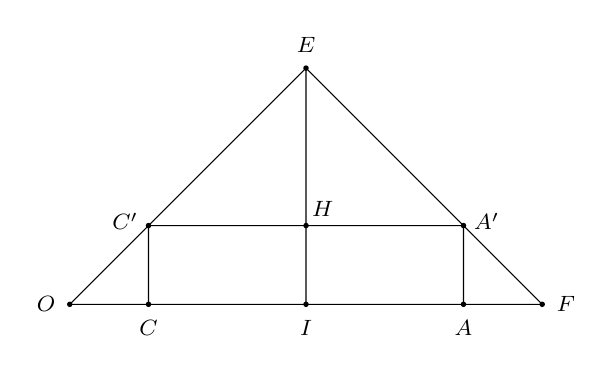
\begin{tikzpicture}[scale=1,>=stealth, font=\footnotesize, line join=round, line cap=round]
		\path%Khai báo các điểm
		(0:0) coordinate (O)--++(0:1)coordinate (C)--++(90:1)coordinate (C1)
		(0:6) coordinate (F)--++(180:1)coordinate (A)--++(90:1)coordinate (A1)
		(0:3) coordinate (I)--++(90:3) coordinate (E) 
		(intersection of O--E and C--C1) coordinate (C')
		(intersection of F--E and A--A1) coordinate (A')
		(intersection of I--E and A'--C') coordinate (H)
		;
		\draw (O)--(E)--(F)--(O) (I)--(E) (C)--(C')--(A')--(A);
		\foreach \x/\g in {O/180,F/0,I/-90,C/-90,A/-90,C'/170,A'/10,E/90,H/45}\fill[black] (\x) circle (1pt) +(\g:.3)node{$\x$};
		\end{tikzpicture}
	\end{center}
	Xét phần mặt cắt qua trục hình nón và đi qua mặt phẳng $(AA'C'C)$, kí hiệu như hình vẽ. Với $I,H$ lần lượt là tâm của hình vuông $ABCD$, $A'B'C'D'$ và đỉnh $A'$ nằm trên đường sinh $EF$ của hình nón.\\
	Hình lập phương có thể tích bằng $1$ nên $AA'=HI=1$, $A'H=\dfrac{\sqrt{2}}{2}$.\\
	Đặt $EH=x$ $(x>0)$. Khi đó, ta có
	$$\dfrac{EH}{EI}=\dfrac{A'H}{FI} \Leftrightarrow \dfrac{x}{x+1}=\dfrac{\sqrt{2}}{2FI}\rightarrow FI=\dfrac{\sqrt{2}}{2}\left(\dfrac{x+1}{x}\right)=r.$$
	Thể tích khối nón $(N)$ là $V=\dfrac{1}{3} \pi r^2 EI=\dfrac{1}{6} \pi\left(\dfrac{x+1}{x}\right)^2(x+1)=\dfrac{\pi}{6} \dfrac{(x+1)^3}{x^2}$.\\
	Xét hàm số $f(x)=\dfrac{(x+1)^3}{x^2}, \forall x\in (0;+\infty)$. Ta có $f'(x)=\dfrac{(x-2)(x+1)^2}{x^3}$.\\
	Lập bảng biến thiên
	\begin{center}
		
\begin{tikzpicture}
		\tkzTabInit[nocadre=false,lgt=1.5,espcl=3,deltacl=.6]
		{$x$/0.6,$f'(x)$/0.6,$f(x)$/2}
		{$0$,$2$,$+\infty$}
		\tkzTabLine{,-,$0$,+,}
		\tkzTabVar{+/,-/$\dfrac{27}{4}$,+/}
		\end{tikzpicture}
	\end{center}
	Ta được $\min\limits_{(0;+\infty)} f(x)=\dfrac{27}{4}$ tại $x=2$. Suy ra $\min V=\dfrac{9 \pi}{8}$.
}
\end{ex}

\begin{ex}%[Thi thử tốt nghiệp - Liên trường Nghệ An-23]%[Nguyễn Đăng Tuấn - 12-EX6-2023]%[2H3G2-8]
Trong không gian $Oxyz$, cho hình lăng trụ đứng $ABC.A'B'C'$ có $AB=4$, $\widehat{ACB}=150^\circ $. Ba điểm $A$, $B$, $C$ thay đổi nhưng luôn thuộc mặt cầu $(S)\colon x^2+y^2+z^2+8x-6y+4z+4=0$; ba điểm $A'$, $B'$, $C'$ luôn thuộc $(P)\colon x+2y+2z+23=0$. Thể tích lớn nhất của tứ diện $ABC'B'$ bằng
\choice
{\True $\dfrac{40(2-\sqrt{3})}{3}$}
{$\dfrac{24}{4-\sqrt{3}}$}
{$\dfrac{8}{4-\sqrt{3}}$}
{$80(2-\sqrt{3})$}
\loigiai{
	$(S)$ có tâm $I(-4;3;-2)$ và bán kính $R=5$. \\
	Ta có $V_{ABC'B'}=\dfrac{1}{3}{V}_{ABC.A'B'C'}$, nên để thể tích của tứ diện $ABC'B'$ lớn nhất thì thể tích của khối lăng trụ $ABC.A'B'C'$ lớn nhất.\\
	Gọi $r$ là bán kính đường tròn ngoại tiếp tam giác $ABC$, khi đó $r=\dfrac{AB}{2\sin \widehat{ACB}}=\dfrac{4}{2\sin 150^\circ}=4$.\\
	Khi đó, ta có $\mathrm{d}(I,(ABC))=\sqrt{R^2-r^2}=3$ suy ra khoảng cách lớn nhất của hai mặt phẳng chứa hai đáy hình trụ là $\mathrm{d}(I,(ABC))+\mathrm{d}(I,P)=10$.
	\begin{center}
		\begin{tikzpicture}[scale=1,>=stealth, font=\footnotesize, line join=round, line cap=round]
		\path%Khai báo các điểm
		(0:0) coordinate (E)
		(60:3) coordinate (B)
		(120:3) coordinate (A)
		(90:3) coordinate (C)
		($(A)!.5!(B)$) coordinate (H)
		;
		\draw (E) circle(3 cm);
		\draw (A)--(B)--(E)--(A)--(C)--(B) (C)--(E);
		\foreach \x/\g in {A/170,B/10,C/90,H/-135,E/-90}\fill[black] (\x) circle (1pt) +(\g:.3)node{$\x$};
		\end{tikzpicture}
	\end{center}
	Gọi $E$ là tâm đường tròn ngoại tiếp tam giác $ABC$.\\
	Ta có $AB=4=r$ nên tam giác $ABE$ đều. Gọi $H$ là trung điểm $AB$.\\
	Ta có $S_{ABC}$ lớn nhất khi khoảng cách từ $C$ đến $AB$ lớn nhất hay $E$, $H$, $C$ thẳng hàng.\\
	Khi đó $CH_{\max}=CE-HE=4-2\sqrt{3}$ $\Rightarrow V_{ABC'B'}=\dfrac{1}{3}{V}_{ABC.A'B'C'}=\dfrac{1}{3}\mathrm{d}\left((ABC),(A'B'C')\right)\cdot S_{ABC}$\\
	$\Rightarrow V_{ABC'B'}=\dfrac{1}{3}\cdot 10\cdot \dfrac{1}{2}\cdot 4\cdot (4-2\sqrt{3})=\dfrac{40(2-\sqrt{3})}{3}$.
}
\end{ex}

\begin{ex}%[Thi thử tốt nghiệp - Liên trường Nghệ An-23]%[Nguyễn Đăng Tuấn - 12-EX6-2023]%[2H3G2-3]
Trong không gian $Oxyz$, cho điểm $H(a;2;5)$. Mặt phẳng $(P)$ đi qua điểm $H$ cắt các trục tọa độ $Ox$, $Oy$, $Oz$ lần lượt tại $A$, $B$, $C$ sao cho $H$ là trực tâm của tam giác $ABC$. Biết rằng, $(P)$ song song với đường thẳng đi qua hai điểm $M(3;1;7)$ và $N(7;4;5)$. Phương trình $(P)$ là
\choice
{\True $x+2y+5z-30=0$}
{$2x+4y+10z-2=0$}
{$x+2y+5z+30=0$}
{$2x+4y-10z+1=0$}
\loigiai{
	\begin{center}
		\begin{tikzpicture}[scale=1,>=stealth, font=\footnotesize, line join=round, line cap=round]
		\path%Khai báo các điểm
		(0:0) coordinate (O)
		(-30:2) coordinate (C)
		(-160:3) coordinate (B)
		(90:3) coordinate (A)
		($(C)!.5!(B)$) coordinate (E)
		($(C)!.5!(A)$) coordinate (F)
		(intersection of A--E and B--F) coordinate (H)
		;
		\draw (A)--(B)--(C)--(A)--(E) (B)--(F) ;
		\draw[dashed] (A)--(O)--(B) (H)--(O)--(C);
		\foreach \x/\g in {A/90,B/180,C/0,F/20,E/-90,H/180,O/0}\fill[black] (\x) circle (1pt) +(\g:.3)node{$\x$};
		\draw pic[draw,angle radius=2mm]{right angle=A--E--C};
		\draw pic[draw,angle radius=2mm]{right angle=B--F--C};
		\draw pic[draw,angle radius=2mm]{right angle=B--O--C};
		\end{tikzpicture}
	\end{center}
	\textbf{Bổ đề:} Cho hình chóp $OABC$ có $OA$, $OB$, $OC$ đôi một vuông góc với nhau. Nếu $H$ là trực tâm tam giác $ABC$ thì $OH\perp (ABC)$.\\
	\textbf{Chứng minh:} Kẻ hai đường cao $AE$, $BF$ cắt nhau tại $H$ của tam giác $ABC$.\\
	Ta có $\heva{&AE\perp BC \\&AO\perp BC} \Rightarrow BC\perp (AEO)\Rightarrow BC\perp OH$ và $\heva{&BF\perp AC \\&BO\perp AC}\Rightarrow AC\perp (BFO)\Rightarrow AC\perp OH$
	$\Rightarrow OH\perp (ABC)$.\\
	Áp dụng bổ đề trên ta $\overrightarrow{n}_P=\overrightarrow{OH}=(a;2;5)$$\Rightarrow (P)\colon ax+2y+5z-a^2-29=0$.\\
	Mà $MN \parallel (P)\Rightarrow \overrightarrow{MN}\cdot \overrightarrow{OH}=0\Leftrightarrow 4a+6-10=0\Leftrightarrow a=1$.
	Vậy $(P):x+2y+5z-30=0$.
}
\end{ex}
\Closesolutionfile{ans}
\begin{indapan}{10}
	{ans/ans-2-TT-9-LienTruongNgheAn-23}
\end{indapan}